%Master File:lectures.tex

\lesson{Gene Regulation Networks}
\vspace{-2cm}
\begin{center}
  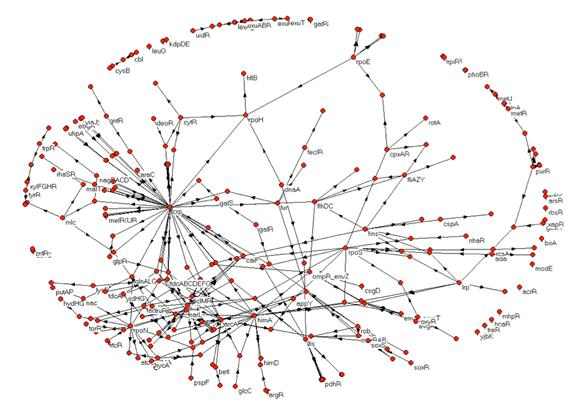
\includegraphics[height=10cm]{figures/ecoliGRN}
\end{center}

\keywords{Gene regulation, chemical equations, motifs}
%%%%%%%%%%%%%%%%%%%%%%% Next Slide %%%%%%%%%%%%%%%%%%%%%%%
\renewcommand{\Outline}{%
\begin{slide}
\section[1]{Outline}

\begin{minipage}{10cm}
  \begin{enumerate}\squeeze
    \outlineitem{Gene Regulation}{genereg}
    \outlineitem{Chemical Equations}{chemeq}
    \outlineitem{Motifs}{motifs}
   \end{enumerate}
\end{minipage}\hfill
\begin{minipage}{12cm}
  \vfill
  
\includegraphics[width=12cm]{GRNcircle}
  \vfill
\end{minipage}
\end{slide}
\addtocounter{outlineitem}{1}
}

\setcounter{outlineitem}{1}
\Outline
\toptarget{firstoutline}
%%%%%%%%%%%%%%%%%%%%%%% Next Slide %%%%%%%%%%%%%%%%%%%%%%%

\begin{slide}
\section{Transciption Networks}

\begin{PauseHighLight}
  \begin{itemize}
  \item Signalling molecules combine with transcription factors
    (proteins) which excite or inhibit the transcription of other proteins\pause
  \end{itemize}
  \begin{center}
    
\includegraphics[width=0.9\linewidth]{transciptionNetwork}
  \end{center}
\end{PauseHighLight}

\end{slide}

%%%%%%%%%%%%%%%%%%%%%%% Next Slide %%%%%%%%%%%%%%%%%%%%%%%

\begin{slide}
\section[-2]{Gene Transcription Regulation}
\pause
\pb \pauselevel{=1}
\begin{center}
  \multipdf[width=\linewidth]{geneTranReg}\pause
\end{center}

\end{slide}

%%%%%%%%%%%%%%%%%%%%%%% Next Slide %%%%%%%%%%%%%%%%%%%%%%%

\begin{slide}
\section{Time Scales}

\begin{PauseHighLight}
  \begin{itemize}
  \item Reactions happen on different time scales
    \begin{itemize}
    \item Binding of small (signalling) molecules: \hfill $\sim1$ msec\quad\pause
    \item Binding of active transcription factor: \hfill $\sim1$ sec\quad\pause
    \item Transciption + translation of gene: \hfill $\sim5$ min\quad\pause
    \item 50\% change in concentration of protein: \hfill $\sim1$ hour\quad\pause
    \end{itemize}
  \item We can assume all events at earlier time scales happen instantly\pause
  \end{itemize}
\end{PauseHighLight}


\end{slide}

%%%%%%%%%%%%%%%%%%%%%%% Next Slide %%%%%%%%%%%%%%%%%%%%%%%
\Outline % Chemical Equations
%%%%%%%%%%%%%%%%%%%%%%% Next Slide %%%%%%%%%%%%%%%%%%%%%%%

\newcommand{\RNA}{\mathit{RNA}}

\begin{slide}
\section{Chemical Equations}

\begin{PauseHighLight}
  \begin{itemize}
  \item We can write down the mechanism that underlie gene regulation in
    terms of chemical equations
    \begin{align*}
      X &\stackrel{k_1}{\longrightarrow} X + \RNA_Y \\
      \RNA_Y &\stackrel{k_2}{\longrightarrow} \RNA_Y + Y \\
      \RNA_Y &\stackrel{k_3}{\longrightarrow} \varnothing\pause
    \end{align*}
  \item These are massively simplified (but we can ignore reactions that
    happen quickly)\pause
  \item The rate of reaction depends on the number/concentration of the
    molecules on the left-hand side and the reaction rate $k_i$\pause
  \end{itemize}
\end{PauseHighLight}

\end{slide}

%%%%%%%%%%%%%%%%%%%%%%% Next Slide %%%%%%%%%%%%%%%%%%%%%%%

\begin{slide}
\section[-2]{Changes on Average}

\begin{PauseHighLight}
  \begin{itemize}
  \item Chemical equations happen at random, so the rate equations
    describe the average changes
    \begin{align*}
      X &\stackrel{k_1}{\longrightarrow} X + \RNA_Y \\
      \RNA_Y &\stackrel{k_2}{\longrightarrow} \RNA_Y + Y \\
      \RNA_Y &\stackrel{k_3}{\longrightarrow} \varnothing\pause
    \end{align*}
  \item Let $[X]$ denote the (mean) concentration of $X$ then
    \begin{align*}
      \frac{\dd [\RNA_Y]}{\dd t} &= k_1 \, [X] - k_3\,  [\RNA_Y] \\
      \frac{\dd [Y]}{\dd t} &= k_2 \, [\RNA_Y]\pause
    \end{align*}
  \end{itemize}
\end{PauseHighLight}

\end{slide}


%%%%%%%%%%%%%%%%%%%%%%% Next Slide %%%%%%%%%%%%%%%%%%%%%%%

\begin{slide}
\section{Reaction Rates and Concentrations}

\begin{PauseHighLight}
  \begin{itemize}
  \item When we consider reaction involving multiple molecular species,
    e.g. two proteins forming a complex
    \begin{align*}
      X + Y \stackrel{k_4}{\longrightarrow} C\pause
    \end{align*}
  \item The reaction rates depend on concentrations of $X$ and $Y$ (how
    likely is it for two molecules to collide)\pause
  \item To find the concentration we have to divide by the volume of the
    cell, $V$\pause
  \item To obtain concentrations in moles (we also have to divide by
    Avogadro's number $A$)\pause
  \end{itemize}
\end{PauseHighLight}

\end{slide}

%%%%%%%%%%%%%%%%%%%%%%% Next Slide %%%%%%%%%%%%%%%%%%%%%%%

\begin{slide}
\section{Changes on Average}

\begin{PauseHighLight}
  \begin{itemize}
  \item Thus
    \begin{align*}
      X + Y \stackrel{k_4}{\longrightarrow} C\pause
    \end{align*}
  \item Implies on average
    \begin{align*}
      \frac{\dd [X]}{\dd t} = \frac{\dd [Y]}{\dd t}
      &= -k_4 \, [X]\,[Y] \pause
      &&&
        \frac{\dd X}{\dd t} = \frac{\dd Y}{\dd t}
      &= -\frac{k_4}{\Omega} \, X\,Y \pauseb
      \\
      \frac{\dd [C]}{\dd t}
      &= k_4 \, [X]\,[Y]\pauselevel{=2} \pause
      &&& \frac{\dd C}{\dd t}
      &= \frac{k_4}{\Omega} \, X\,Y\pauselevel{=3}
    \end{align*}  
  \item $\Omega=V A$, $[X]=X/\Omega$ and $[Y]=Y/\Omega$\pauseb
  \end{itemize}
\end{PauseHighLight}

\end{slide}




%%%%%%%%%%%%%%%%%%%%%%% Next Slide %%%%%%%%%%%%%%%%%%%%%%%

\begin{slide}
\section{Fluctuations}

\begin{PauseHighLight}
  \begin{itemize}
  \item In chemistry we are used to there being so many molecules that
    the average rate equations provide a very good approximation of what
    really happens\pause
  \item This is often true in biology, but not always\pause
  \item Cells are small and some proteins can occur in very small
    numbers\pause
  \item We return to the problem of modelling systems with small number
    of molecules in the last lecture\pause
  \item For the time being we take the differential equation model as
    an accurate description of our gene regulation network\pause
  \end{itemize}
\end{PauseHighLight}

\end{slide}

%%%%%%%%%%%%%%%%%%%%%%% Next Slide %%%%%%%%%%%%%%%%%%%%%%%

\begin{slide}
\section{Switches}

\begin{PauseHighLight}
  \begin{itemize}
  \item Our molecular equation depend on the product of concentrations
    of the components on the left-hand side\pause
  \item This can lead to strong non-linearities\pause
  \item Such non-linearity can simulate switch like mechanism\pause
  \item This is often useful for robust regulation\pause
  \end{itemize}
\end{PauseHighLight}

\end{slide}

%%%%%%%%%%%%%%%%%%%%%%% Next Slide %%%%%%%%%%%%%%%%%%%%%%%

\begin{slide}
\section{Signalling}

\begin{PauseHighLight}
  \begin{itemize}
  \item We showed earlier that proteins are often \textit{activated} by
    signalling molecules combining with the protein to form a
    complex\pause
  \item Proteins can have multiple sub-units that each bind with a
    signalling molecule\pause
  \item A complex might only be stable when the protein has bound some
    number of signalling molecules\pause
  \end{itemize}
\end{PauseHighLight}

\end{slide}

%%%%%%%%%%%%%%%%%%%%%%% Next Slide %%%%%%%%%%%%%%%%%%%%%%%

\begin{slide}
\section[-2]{Multi-signalling}

\pause\pb\pauselevel{=1}
\begin{center}
  \multipdf[width=0.9\linewidth]{HillEquation}\pause
\end{center}
\end{slide}

%%%%%%%%%%%%%%%%%%%%%%% Next Slide %%%%%%%%%%%%%%%%%%%%%%%
\newcommand{\koff}{k_{\text{\tiny\it off}}}
\newcommand{\kon}{k_{\text{\tiny\it on}}}

\begin{slide}
\section[-2]{Hill Equation}

\pb
\begin{itemize}
\item We assume that we form a complex with $n$ signalling molecules
  $S_X$
  \begin{align*}
    n\, S_X + X &\stackrel{\kon}{\longrightarrow} C
    &
      C &\stackrel{\koff}{\longrightarrow} n\, S_X + X \pauseh
  \end{align*}
\item Which we can model using
\end{itemize}
  \begin{center}
    \multipdf[width=\linewidth]{hillEq}\pause
  \end{center}

\end{slide}


%%%%%%%%%%%%%%%%%%%%%%% Next Slide %%%%%%%%%%%%%%%%%%%%%%%

\begin{slide}
\section[-2]{Hill Coefficient}

\pb
{\small \begin{align*}
  \frac{[C]}{[X_T]} = \frac{[S_X]^n}{K_X^n + [S_X]^n}\pauseh
\end{align*}}
\pauselevel{=1}
\begin{center}
  \multipdf[width=0.85\linewidth]{hillCurves}\pause
\end{center}

\end{slide}

%%%%%%%%%%%%%%%%%%%%%%% Next Slide %%%%%%%%%%%%%%%%%%%%%%%

\begin{slide}
\section[-2]{Activator and Repressor}

\pb
\begin{minipage}{0.66\linewidth}
  \begin{itemize}
  \item A protein that acts to increase the expression of a protein we
    call an \emph{activator}\pauseh
  \item The activation coefficient is often given by the Hill-equation
    \begin{align*}
      f([X]) = \frac{\beta \,[X]^n}{K^n + [X]^n}\pauseh
    \end{align*}
  \item By a similar argument a protein that acts as a \emph{repressor}
    is given by
    \begin{align*}
      f([X]) = \frac{\beta}{1+([X]/K)^n}\pauseh
    \end{align*}
  \end{itemize}
\end{minipage}\hfil
\begin{minipage}{0.33\linewidth}
  \begin{center}
    \multipdf[width=0.99\linewidth]{activator}\pause \\
    \multipdf[width=0.99\linewidth]{repressor}\pause
  \end{center}
\end{minipage}


\end{slide}



%%%%%%%%%%%%%%%%%%%%%%% Next Slide %%%%%%%%%%%%%%%%%%%%%%%
\Outline % Motifs
%%%%%%%%%%%%%%%%%%%%%%% Next Slide %%%%%%%%%%%%%%%%%%%%%%%

\begin{slide}
\section{Understanding Gene Regulation Networks}

\begin{PauseHighLight}
  \begin{itemize}
  \item We can infer interactions between proteins as we described in a
    previous lecture\pause
  \item Gene regulation networks tend to be rather complicated\pause
  \item To make sense of them we wish to look for patterns,
    ``\emph{motifs}'', that occur very often\pause
  \item We look at interactions that occur more often than would be
    expected to happens in a random network\pause
  \end{itemize}
\end{PauseHighLight}

\end{slide}

%%%%%%%%%%%%%%%%%%%%%%% Next Slide %%%%%%%%%%%%%%%%%%%%%%%

\begin{slide}
\section[-2]{E-Coli GRN}

\begin{center}
  
\includegraphics[width=0.9\linewidth]{ecoliGRN}
\end{center}
\end{slide}

%%%%%%%%%%%%%%%%%%%%%%% Next Slide %%%%%%%%%%%%%%%%%%%%%%%

\begin{slide}
\section[-2]{Auto-regulation}

\begin{PauseHighLight}
  \begin{itemize}
  \item In E-coli we have $N=424$ nodes and $E=519$ edges\pause
  \item The total number of directed edges (including self-edges) is
    $N^2$\pause
  \item The number of self edges is $N$ so the probability of a randomly
    chosen edge being a self-edge is $p=1/N$\pause
  \item The probability that if we choose $E$ edges $k$ will be
    self-edges is
    \begin{align*}
      \Prob{k|E,p} = \mathrm{Binom}(k|E,p) = \binom{E}{k}\,p^k\,(1-p)^{E-k}\pause
    \end{align*}
  \item This has mean $\av{N_{\text{\tiny self}}} = E\,p \approx 1.2$ and
    standard deviation $\sigma = \sqrt{E\,p\,(1-p)} \approx 1.1$\pause
  \item In fact we have $N_{\text{\tiny self}}=40$\pause{} (that is, $32\,\sigma$
    above the mean)\pauseb
  \end{itemize}
\end{PauseHighLight}

\end{slide}

%%%%%%%%%%%%%%%%%%%%%%% Next Slide %%%%%%%%%%%%%%%%%%%%%%%

\begin{slide}
\section[-1]{No Auto-Regulation}

\begin{PauseHighLight}
  \begin{itemize}
  \item To understand why auto-regulation is interesting let us first
    consider the case with no negative feedback\pause
  \item We assume
    \vspace*{-2cm}
    \begin{align*}
      \varnothing &\stackrel{\hat{\beta}}{\longrightarrow} \hat{X} \\
      \hat{X} &\stackrel{\hat{\alpha}}{\longrightarrow} \varnothing\pause
    \end{align*}
  \item So on average
    \vspace*{-1cm}
    \begin{align*}
      \frac{\dd [\hat{X}]}{\dd t} = \hat{\beta} - \hat{\alpha}\, [\hat{X}]\pause
    \end{align*}
  \item This has a steady state $[\hat{X}_{eq}] = \hat{\beta}/\hat{\alpha}$\pause
  \end{itemize}
\end{PauseHighLight}

\end{slide}

%%%%%%%%%%%%%%%%%%%%%%% Next Slide %%%%%%%%%%%%%%%%%%%%%%%

\begin{slide}
\section[-1]{Solving Differential Equations}

\begin{PauseHighLight}
  \begin{itemize}
  \item The full dynamics is given by the solution to the differential
    equation and depend on the initial condition, $[\hat{X}(0)]$\pause
  \item Most differential equations cannot be solved in closed
    form\pause
  \item However, they are usually quite easy to solve numerically
    (though it is difficult to understand how the solution depend on the
    parameters)\pause
  \item Our equation is linear and is easy to solve.\pause{}  For $[\hat{X}(0)]=0$
    \begin{align*}
      \frac{\dd [\hat{X}(t)]}{\dd t} &= \hat{\beta} - \hat{\alpha}\,[\hat{X}(t)]
      & &\Rightarrow&
     [\hat{X}(t)] &= \frac{\hat{\beta}}{\hat{\alpha}}
                      \left( 1- \e{-\hat{\alpha}\,t} \right)\pause
    \end{align*}
  \end{itemize}
\end{PauseHighLight}

\end{slide}

%%%%%%%%%%%%%%%%%%%%%%% Next Slide %%%%%%%%%%%%%%%%%%%%%%%

\begin{slide}
\section[-2]{Auto-regulation}

\begin{PauseHighLight}
  \begin{itemize}
  \item We assume a negative feedback so that
    \begin{align*}
      \frac{\dd [X]}{\dd t} = f([X]) - \alpha \, [X]\pause
    \end{align*}
  \item Where we have a Hill-type repressor
    \begin{minipage}{0.78\linewidth}
      \begin{align*}
        f([X]) = \frac{\beta}{1 + ([X]/K)^n} \approx \beta\,\pred{[X]<K} 
      \end{align*}
    \end{minipage}\hfil
    \begin{minipage}{0.20\linewidth}
      
\includegraphics[width=1.1\linewidth]{repressor-3}\pause
    \end{minipage}
  \item Starting from $[X(0)]=0$ initially $[X(t)]=\beta\,t$\pause
  \item When $[X(t)]>K$ then $f([X(t)])=f(K+\epsilon)\approx 0$ and a steady state is
    reached\pause 
  \end{itemize}
\end{PauseHighLight}

\end{slide}

%%%%%%%%%%%%%%%%%%%%%%% Next Slide %%%%%%%%%%%%%%%%%%%%%%%

\begin{slide}
\section{Controlled Comparison}

\begin{PauseHighLight}
  \begin{itemize}
  \item To compare to having no feedback we want our two circuits to be
    as similar as possible\pause
  \item Choose the same decay rate $\alpha=\hat{\alpha}$\pause
  \item Choose $K = \hat{\beta}/\hat{\alpha}$ so that the steady state
    or equilibrium value of $X(t)$ is the same in both
    systems $[\hat{X}_{eq}]=[X_{eq}]$\pause
  \item Note that in the auto-regulation system the rate of production
    $\beta$ is decoupled from the steady-state\pause
  \end{itemize}
\end{PauseHighLight}

\end{slide}

%%%%%%%%%%%%%%%%%%%%%%% Next Slide %%%%%%%%%%%%%%%%%%%%%%%

\begin{slide}
\section[-2]{$\beta=2$}
\pause\pb\pauselevel{=1}
\begin{center}
  \multipdf[width=0.8\linewidth]{autoRegulation}\pause
\end{center}
\end{slide}


%%%%%%%%%%%%%%%%%%%%%%% Next Slide %%%%%%%%%%%%%%%%%%%%%%%

\begin{slide}
\section{Advantages of Auto-regulation}

\begin{PauseHighLight}
  \begin{itemize}
  \item Auto-regulation allows us to use a large production rate $\beta$
    for the same equilibrium, speeding up the equilibration time\pause
  \item Note that we can independent evolve $K$ (by mutations to the
    binding site of $X$ in the promoter region) and $\beta$, by
    mutations in the binding site of RNA polymerase\pause
  \item Another advantage is that $\beta$ and $\alpha$ can strongly
    fluctuate during the life time of a cell caused by fluctuations in
    metabolic capacity\pause
  \item $K$ depends on the chemical bonds in the binding site and is
    typically more stable\pause
  \end{itemize}
\end{PauseHighLight}

\end{slide}

%%%%%%%%%%%%%%%%%%%%%%% Next Slide %%%%%%%%%%%%%%%%%%%%%%%

\begin{slide}
\section{Summary}

\begin{PauseHighLight}
  \begin{itemize}
  \item We can begin to understand some of the gene regulation dynamics
    by writing down chemical equations\pause
  \item We can express the mean change in number of molecules through
    differential equations\pause
  \item We can find common motifs, by looking for patterns that occur in
    GRN more often than we would expect in a random network\pause
  \item One common motif is negative auto-regulation (negative feedback)
    that allows us to increase the response rate to reach the same
    equilibrium level of a molecule\pause
  \end{itemize}
\end{PauseHighLight}

\end{slide}
